\openingarticle
\def\ppages{\pagerange{Johnson:firstpage}{Johnson:lastpage}}
\def\shorttitle{Interview: Rosemary Joyce}
\def\shortauthor{Lisa M. Johnson}
\def\authormail{llomitola@berkeley.edu}
\def\maintitle{Rosemary Joyce, Ph.D. \textit{Professor of Anthropology at the University of California, Berkeley}}
\def\affiliation{University of California, Berkeley}
%--------------------------------------------------------------
\mychapter{Rosemary Joyce, Ph.D.\newline \textit{Professor of Anthropology at the University of California, Berkeley}}
\begin{center}
	{\Large\scshape\shortauthor}\\[1em]
	\email \\
	\affiliation
\end{center}
\vspace{3em}
\midarticle
%--------------------------------------------------------------
 \label{Johnson:firstpage}
 	
	%----------------------------------------------------------------------------------------
	%	ARTICLE CONTENTS
	%----------------------------------------------------------------------------------------

\SetBlockThreshold{1} 
\blockquote{Throughout my time as a university level student, I have had the opportunity to learn from some very successful Maya scholars with years of field and research experience.  So I understand how crucial and formative those years are for beginning university students in developing as independent thinkers, writers and field archaeologists.  When I was asked to conduct an interview with my advisor and mentor, Dr. Rosemary Joyce, I was more than happy to do so.  She is a passionate educator and influential anthropologist that I believe is a great person to include in the first issue of the \textbf{\textit{International Journal of Student Research in Archaeology}}. -- L.M. Johnson}	
	
	\begin{figure}
		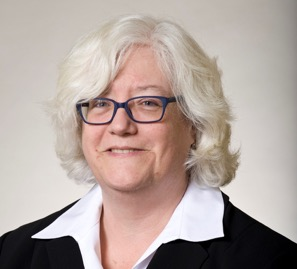
\includegraphics[width=.75\linewidth]{figures/johnson_fig1}
		\centering
		\caption{Rosemary Joyce, Ph.D., Professor of Anthropology at the University of California, Berkeley}
		\label{fig:Johnson:Fig1}
	\end{figure}
	
\begin{labeling}{IJSRA}
	\item[IJSRA (International Journal of Student Research in Archaeology)] \textit{You have often been an advocate for undergraduate research and writing, enabled through very specific learning settings and curriculum structure.  Can you briefly discuss your philosophy of teaching, learning and practice?}
	
	\item[RAJ (Dr. Rosemary A Joyce)] I begin with the proposition that learning happens by engaging directly in the closest way possible to professional practice. This draws on the writing of anthropologist Jean Lave, whose concept of "Legitimate Peripheral Participation" says that we learn when what we do is legitimate, not a made up exercise, as long as what we are asked to do is something we can successfully do with the skills we have at our stage of practice. The example in her collaborative book (with sociologist Etienne Wenger) Situated Learning of tailors in west Africa stuck with me: she noted that novices are given jobs like finishing buttonholes, which is reversible (if they do it wrong) and won't wreck the piece of clothing. Only after you gain greater skill do you get to cut the cloth into pieces. 
	
	So what's the equivalent in teaching? Right away, I realized that the conventional term paper-- write 25 pages at the end of a semester-- is not what Lave and Wenger are promoting. Instead, in each course, I ask, what do beginning scholars do to gain skills? So an early assignment may be a book review; or writing an annotated entry for a bibliography; or working in a group to develop a grant proposal. In my museum exhibit design course, for example, instead of having the class develop and install an exhibit in one semester-- something that isn't true to museum practice-- we spend the semester identifying the audience for an exhibit, developing themes, writing sample texts, doing layouts-- and assemble those things in a draft following the guidelines of the NEH.
	
	What goes along with this actively engaged approach to learning is that each student is responsible for learning. I have no way to pour coins of knowledge into someone's head-- the discredited but still all too alive banking model. Learners create their own knowledge. So in large lecture courses, I try to set things up so that students discuss readings and reach their own understandings before I tell them my opinions about the topic. This means my lectures follow from what students raise as questions and concerns. Every time I teach a course, my lectures are different, because each group of students starts at its own point, and develops at its own pace. I have had to move to defining semester-long goals and sets of concepts I want to be sure to cover-- and to be prepared to talk about those when the students want, not when I would prefer.

\item[IJSRA] \textit{You have been engaging with fieldwork in Honduras since 1977. What kind of research are you carrying out, and what opportunities and challenges are still present for students interested in Mesoamerican archaeology?}

\item[RAJ] In 2009, there was a coup in Honduras. Since then, I have not returned to fieldwork there; instead, I returned to my original love, museum work, and have now travelled to museums throughout Europe and the US to record older museum collections from Honduras and begin to do what we keep saying we as a discipline need to do: excavate the museums. This has led to my series of projects about materiality, how things created social relations, drawing from study of museum collections and pulling together data from field projects.

  I have encouraged students to consider when already existing collections may be the right thing for them to use to address a specific question: after all, we are a problem-oriented discipline, and where our data lie follows from the questions we ask. I have had recent PhD students I co-advised (our normal model at Berkeley) who studied human remains from colonial Mexico City, and the metal objects from the Cenote of Sacrifice at Chichén Itzá.
  
  Still, many of my grad students do conduct original excavations as part of their dissertation projects. Since 2010, I have been lucky to have a great collaboration with a leading Mexican Maya specialist, Rodrigo Stuardo Liendo, a senior researcher from \textit{Universidad Nacional Autonoma de México} (UNAM), who spent a year at Berkeley on sabbatical a while back, and so current and former students of mine are engaged in household archaeology, the study of ritual, and archaeologies of practice and materiality in Chiapas.
  
 What I see as a major challenge for students starting out in Mesoamerican archaeology is simply that it is no longer feasible to conduct as much fieldwork as people in my generation were able to do for a dissertation. I spent about 20 months total in the field working on my dissertation. That was possible in part because it was relatively inexpensive to work in Honduras, and partly because many of the methods in general use now were not even developed then, or were only done by specialists. Today, the goal is quality of data, employing a range of analyses to tease out more information, even from the sediments (through micromorphology, for example), rather than quantity, which was key to research questions in the 1970's that aimed to generalize about life in specific sites from a dissertation research project. So archaeology today requires a different kind of research question. But we haven't switched gears quite quickly enough: I often read proposals for dissertation research that propose to make broad interpretations from small samples, and that really doesn't work.

\item[IJSRA] \textit{Considering your academic trajectory (B.A. Cornell, PhD Illinois-Urbana, Harvard, Berkeley), does the US system encourage mobility and academic exchange, in contrast with the life-long attachment of academics to their alma maters in other countries? In 1994, you joined the Anthropology Department at Berkeley from Harvard. What attracted you the most about UC Berkeley?}

\item[RAJ] Mobility is relative: the US has such a large number of universities, especially state universities, that it can look like people are flowing all around. But since moving to California, I have been struck by how this apparent circulation conceals some circuits. We know from research done at Berkeley that the majority of Berkeley PhDs across all fields who pursue academic careers stay on the west coast, the vast majority, in California itself. I don't think my own trajectory is a model; it is more testimony to the role of accident in the absence of knowledge about how academia works. I am a first generation college graduate (neither of my parents graduated from college). My working class family had no tradition of postgraduate education for me to draw on; although one of my brothers has an MFA and is also a college professor, I was the only PhD in my immediate family at the time that I received the degree. So at each step, I kind of fell into where I went. Cornell was recommended to me by a doctoral candidate who was employed in education programs at the Buffalo Museum of Science, where I worked as a volunteer; she had gone to ASU and regretted not trying to get into an Ivy League school. But Cornell was a bad choice for me at the time, since my original goal was to do historical archaeology of the 19th century US-- preferably New York State. Mesoamerica was an accident due to a field school opportunity (actually, of course, I went to the Naco Valley in Honduras, which is not core Mesoamerica). When it came time to apply to grad schools, my approach was pretty unsystematic. I asked one grad student on the Naco project where I could go to study Honduran archaeology, having fallen deeply in love with the country, and was told the only person doing a Honduras PhD was at the University of Illinois. I applied there (and a random assortment of places whose names I knew-- Michigan, Chicago, SUNY Albany...). The professor who became my advisor, Dave Grove, made coming to UIUC compelling because he wrote to me personally and explained what I could do there with my career goal-- which was museum work. But it wasn't like he was a specialist in Honduran archaeology.

The job search, of course, was primarily about where the jobs were. I like to tell the story of one of my brothers trying to wrap his head around the idea that I was turned down by University of Wisconsin Lacrosse then hired by Harvard... of course, that was as a museum curator. 

Coming to Berkeley was the first completely intentional move in the trajectory. Harvard at the time did not routinely promote to tenure; I was an untenured Associate Professor, and I really wanted to return to the Chicago area, but the only job open was untenured Assistant Professor. Before that job decided who to interview, Berkeley made me the offer-- and what it offered was a chance to follow up on my work at Harvard's Peabody Museum with directing another of the great anthropology museums in the US.
	
\item[IJSRA] \textit{You are a former curator of the Peabody Museum, Harvard and a former Director of the Hearst Museum of Anthropology, Berkeley. Are Museums effective institutions for the transmission of knowledge and information to anthropology and archaeology students and visitors? What roles should they fulfil? How should they adapt to the new requirements of the 21st century?}

\item[RAJ] Museums are certainly effective-- but they may be effective at creating knowledge that scholars don't want to advance. If you have never worked in a museum, it is easy to think they are traditional and not forward looking. Museum anthropologists actually have been concerned with how to promote engagement, active learning, and how to persuade visitors to reconsider their taken for granteds for a long time-- my entire career, certainly. But the challenge is, museums are settings to which visitors bring their own expectations, their already existing ideas about what is true, and ethnographic research shows they find the parts of museum representations that resonate with their existing knowledge. Museums are nonlinear, so they have the same challenge as the internet-- you cannot ensure that someone reads an introduction before plunging into things. So the process of setting up background knowledge can be daunting. But museums are amazing for the same reason: visitors can literally create unexpected concepts not previously considered. What we need to do is build on what we understand about how people create knowledge in fragments. One practice of some museums that is really useful, and should be universal, is having texts signed by their authors. That is a very modest step toward alerting a visitor that what they are being told is not universal timeless truth, but a representation, an interpretation. If you can then introduce the authors as part of the exhibit, and have multiple authors from different perspectives-- you can open up the idea of museum as laboratory. At the Hearst Museum, my absolute favorite exhibition project was the first one that was developed after I became director: The Carver's Art of the Indians of Northern California. It did all of these things. It also blurred the line between fine art and artifact (including works by modern California Indian artists, one of whom was a co-curator of the exhibit). And it took all the formats possible: a movie, a book, the exhibition, and live programming.	

\item[IJSRA] \textit{In 2001 you contributed to the establishment of the Journal of Social Archaeology. What was the collective motivation behind this new Journal? How would you define “Social Archaeology” and what is the value of researching issues such as gender, household organisation, bodily practices and inter-personal relationships in the past? Why is it important to publish research results, and what role can students play in this process?}

\item[RAJ] Lynn Meskell, the editor in chief, and Bob Preucel, who had been my colleague at Harvard, invited me to be part of the initial editorial panel for the journal. I was enthusiastic, because as I said to them, we needed a place where our students could publish the kinds of cross-disciplinary work that engaged with social theory that we were fostering. At the time, that kind of work could make publishing in journals an uphill battle. I was also enthusiastic about the aim of being international, especially of reaching out to areas, like Latin America, where scholars were doing great work that mainstream English language archaeologists did not always read or cite.

The hardest thing we had to do was craft an editorial statement that clarified what we meant by "social archaeology". If we were writing it today of course, it would be a different statement. But what we wanted to emphasize was centering attention on "the social", which I think of in contrast to the cultural emphasis that remains, even in very processual Americanist work, a dominant strand. To ask questions about how people make histories, how histories make societies, how things make people, all at once: that for me is essentially to address the social. 

It is urgent that all the aspects of social life in the past that can be approached-- which I think is everything, I do not privilege some aspects of social life-- be dealt with. This is a political urgency: so much bad policy in the present world is justified by claiming that there is some natural, or even just long enduring, human way of doing things, archaeologists really need to be vigilant in breaking up that kind of argument. We know that the past is full of alternatives. We need to be sure others don't get away with suggesting any kind of hierarchy, subordination, violence is somehow inevitable.

Publishing research results is a funny topic. First, we need to acknowledge that most archaeological writing reaches tiny audiences. (So does most of any academic discipline, so I am not being harsh about archaeology.) Second, there is a tendency to treat "research results" as little nuggets of information. We need to step back and take a long-overdue look at this topic. First, it is a shame of our discipline-- and I am as guilty as any other active archaeologist-- that we record excavations and excavated material years before we normally produce writing about those records. We could use a return in some ways to a very old form of antiquarian writing, in which descriptive texts (about objects, maps of sites, descriptions of excavations), short narratives, were quickly presented and circulated. The internet means we can do this now and reach millions of people. I recently began a blog called \textit{Real Honduran Archaeology} where participants can just post short reflections-- including short posts that point out material regularities-- without the heavy burden of MAKING A BIG POINT. If we did more of that quick offering of preliminary ideas, we could overcome our disciplinary lag time. But of course, publication has become capital, and only certain kinds of capital count. Also: publishing preliminary ideas means other people may criticize you. And frankly, we have a nasty disciplinary culture that would inhibit most people from taking the risk of saying, "hey, look at these neat data I think might be telling us this...". Too much credit goes to people for the gotcha remark, or even the personal attack. 

I actually think if we could publish descriptions of data more quickly, more informally, with more graceful reception, we would see a huge increase in understanding, because others might recognize connections based on their own experience and knowledge. We could create a network of knowledge production-- which is what I see when I read the 19th century reports that people presented on the antiquities I have been recording in museums. And then, we could each spend the time it takes to mull over the broader implications of our work, we could craft our writing to be beautiful prose that non-archaeologists would read.

So if I could, I would urge students beginning their careers to be generous scholars, to adopt the first person pronoun and hang on to it against all attempts to make you give it up, and to consider developing in parallel works that seek to present observations about archaeological phenomena quickly, and others that seek to intervene in broader public understanding fueled by the expertise that writing about phenomena can develop.

\item[IJSRA] \textit{In 2002 you published The Languages of Archaeology, a book where you analysed the creation of representations of the past by archaeologists. What is the ethical responsibility of archaeological interpretation, and what impact do these creations have in local communities?} 

\item[RAJ] In that book, I argued that archaeologists have a responsibility because even where there are descendant communities, whatever we say based on specific materials we study is a representation that the people represented cannot contest. Their descendants may speak up on their behalf, but we shouldn't be creating that burden. So, as I said there and elsewhere, archaeologists need to acknowledge that history matters, it is political, and we make choices about what aspects of other people's lives we want to foreground. We can sensationalize past societies; we can portray them as failed, as violent, as disappeared; and because of our disciplinary standing, we can do a great deal of damage to the humanity of other people with no (or little) accountability.

This responsibility, for me, is separate from the responsibilities we have to local communities, which we also need to be mindful about. Here, I have a cautious attitude, because sometimes, archaeologists seem to think that we have some special insight to offer, if only the stupid locals understood. To be blunt, we lack humility. So what I think is a useful approach is to seek out the places where archaeological sites are under threat; to labor to create records of those places; and to engage with anyone who expresses an interest in what those places could tell about the past. That may mean-- as it did through most of my years in Honduras-- doing the equivalent of CRM, and finding a way to mold your research orientation to mitigate loss of knowledge during construction. It may mean offering to talk to local groups, but accepting when they don't want you to do so. It means being ready to explain what you are doing and to listen to what people think you should do-- and explain why you cannot if you cannot. Not rocket science, but still not universal: many many archaeological sites are thought of as free from these responsibilities because there are no certified descendant communities, even though there are people living all around.

\item[IJSRA] \textit{An international collaboration between top academics from world-leading universities allowed the publication of the Oxford Handbook of Archaeology (2009), of which you are co-editor. What are for you the positive aspects that such multinational enterprises entail and the issues they encounter?}

\item[RAJ] In 2015, everything is multinational, so it is hard to remember. The biggest goal of opening up debate in archaeology to a global scope (as for example in the JSA, or the series of books that Lynn Meskell and I started for Blackwell) is to mix together people who understand the goals of archaeology very differently: as culture history, as an adjunct to textual history, as cultural heritage, as a branch of social science; and see if it is possible to listen past differences.

\item[IJSRA] \textit{You were appointed in 2011 to the Federal Cultural Property Advisory Committee, advising the State Department of the US on its responses to foreign nations requesting protection of their cultural heritage from looting and antiquities trafficking. How do you think Western countries should deal with issues such as the destruction of national collections and of internationally-recognised and protected sites in the context of armed conflict?}

\item[RAJ] I am happy to serve on the Advisory Committee because it is the means that the US uses to fulfil its obligations to other nations under the UNESCO Convention. But I serve with a real sense of the ambiguity inherent in reinforcing the idea that material remains of the human past should be valued primarily because they are important to national governments. Nationalist strategies draw on materials to put forward a preferred idea of the past that has little to do, in most cases, with the interests and experiences of most people. Indeed, the development of cultural properties for tourism can provide rationales to dislocate and deprive people in the pursuit of a very abstract national identity. This directly underpins the propaganda value that leads to deliberate destruction of material traces of the past, whether in times of armed conflict or as part of development. I wish as archaeologists there were a place for us to stand as critics of the mobilization of things by nations, that would also allow us to decry the pain caused to local people when something they value is destroyed-- I think here of tombs of saints, churches, sacred places valued by indigenous people and endangered by mining. National collections and officially recognized sites are very distant from most people's lives. I am not saying I celebrate such destruction-- there is a legitimate loss to those who love the abstract global past, as all archaeologists do. But even as I support the mobilizations that seek to train US military in how to recognize and protect sites, and the efforts to put in place emergency import restrictions so blood antiquities cannot be trafficked as easily, I think we show a great failure of perspective to worry about these things when so many people have been killed, wounded, and displaced. How would I like to solve this? Stop the wars. Stop strategic invasions. Stop drone strikes. Stop the international traffic in arms. What could we as citizens in "western countries" do? Find a place that is not in flames and help local historians scan photographs. Record gravestones near a community that has no written history before they are lost forever. Spend less of our time pursuing big history, and more writing the textured histories of the local, the everyday, and everyone.

\item[IJSRA] \textit{You are the author of a popular blog \href{https://www.psychologytoday.com/blog/what-makes-us-human}{What Makes Us Human} and you manage an active account on social media, such as Twitter (\href{https://twitter.com/rajoyceucb}{@rajoyceUCB}). What kind of opportunities and challenges does the Internet present for the divulgation of anthropology?}
	
\item[RAJ] I also blog about archaeology at three other places: my own \textit{Ancient Bodies, Ancient Lives}; the collaborative \textit{Real Honduran Archaeology}; and as part of the \textit{Berkeley Blog}, so clearly, I think social media are critical. I actually think we could use social media to renew our discipline. A post I publish on one of these platforms can gain thousands of readers quickly-- not true of a journal article or book. That's the opportunity: to be engaged with wider worlds. The challenges are equally clear: first, we need to relearn how to write for people who are not in the academy or the discipline; second, we need to be prepared to fight for our views-- no one commenting on a blog post really cares that I have a PhD and am a professor at Berkeley if they disagree with me; and third, we need to escape the narratives about archaeology that are waiting to trap us. People know that archaeology is about origins, about discoveries, about treasures, and these are all images that archaeology as a discipline has said we need to erase, and replace. But how do you do that and be interesting as well? I find humor works; so does honest but mild anger (irritation, really). Let people know you care. Tell them why. But mainly, use the same insight I mentioned in writing above about museums: people care about what resonates. Think about how to make something very different seem potentially intelligible to someone unfamiliar with our ideas and methods. Explain our methods! Use everyday language. Use the first person. Write as if archaeology matters in the modern world. 
	
\item[IJSRA] \textit{A 2013 blog entry discusses the importance of funding archaeology. What can archaeological research offer to broader academic debates and how can it contribute to our understanding of the present socio-political reality, in order to remain relevant not only for academic audiences or funding institutions, but also to the wider tax-paying public?}

\item[RAJ]That blog post made an argument that we should not try to bend over backwards to meet the "relevance" criterion, at least as normally envisaged. In that model, we should show how our research helps explain things today. There are places that works-- for example, studies of how people living in arid environments coped and cope today can make very direct comparisons, and historical archaeologists illuminating the emergence of racialism in the US are able to make visible invisible histories that continue to create contemporary conflict and misunderstanding-- but usually, we contort ourselves to be "relevant". I am not able to argue with a straight face that understanding ancient Maya warfare will help us prevent our modern global conflicts. But I can argue that understanding ancient Maya warfare helps us learn how to ask good questions about social life. I actually think the "wider tax-paying public" is more interested in what we have to offer about being human than the logic of relevance, with its implicit utilitarianism, suggests.  I would use the example of talking about gender diversity in the past as a good example: finding instances of same-sex relations doesn't really tell us how to arrange same-sex relationships today. It doesn't compel us to accept marriage equality, nor would the absence of such relationships in the past justify not recognizing them today. But showing that human beings have a diverse history of social arrangements for love, sexuality, reproduction, and economic support is a really good way to show that there is no single way of being human that is more legitimate, universal, or "natural". 

  Archaeologists are in a great position to talk to the public and other disciplines about human variety, flexibility, the plasticity of human behavior, about resilience, about consequences for human abuse of the world. We can show that human societies can fail to meet challenges, because we can show that they have before. And we can show that when human societies fail, it is often because they ignore the evidence before them in order to conserve "traditions" that benefit a few powerful and wealthy individuals. If you want to think of that as relevance, well, OK. But I am not saying we have ever faced the kind of challenge that global warming presents us: I am in fact saying that we have not done so: but we know from other instances in our history that we can kill ourselves through insistence that doing the same thing will work.

  \end{labeling}

\noindent\rule[0.5ex]{\linewidth}{1pt}

\SetBlockThreshold{1} 
\blockquote{Rosemary Joyce, Alice S. Davis Endowed Chair in Anthropology at the University of California, Berkeley, and from 2009 to 2014 the Richard and Rhoda Goldman Distinguished Professor in the Social Sciences, received the PhD from the University of Illinois-Urbana in 1985. A curator and faculty member at Harvard University from 1985 to 1994, she moved to Berkeley in 1994 as Director of the Hearst Museum of Anthropology and a member of the anthropology department. She has been a Fulbright Senior Scholar at the \textit{Universidad de Costa Rica}, as Astor Visiting Lecturer at Oxford University, and a visiting lecturer at Memorial University (Newfoundland), the \textit{Universidad Nacional Autonoma de Mexico}, and the \textit{Universidad de Barcelona}. She has received a John Simon Guggenheim Memorial Foundation Fellowship, and was a Fellow at Radcliffe University's Bunting Institute, the Center for Advanced Study in the Behavioral Sciences at Stanford, and the University of California Humanities Research Institute in Irvine. In 2011 she was appointed by President Barack Obama to the Federal Cultural Property Advisory Committee.}

\SetBlockThreshold{1} 
\blockquote{She is the author of \textit{Cerro Palenque: Power and Identity on the Maya Periphery, Gender and Power in Prehispanic Mesoamerica}, \textit{The Languages of Archaeology}, and \textit{Ancient Bodies, Ancient Lives}, and coauthor of \textit{Embodied Lives} (with Lynn Meskell) and \textit{Material Relations} (with Julia Hendon and Jeanne Lopiparo). For more than thirty-five years she conducted archaeological fieldwork in Honduras, and currently is collaborating in research with Mexican colleagues while continuing research on Honduran collections in European museums.}

	\label{Johnson:lastpage}
%------------------------------------------------------------------------------
\closingarticle